\begin{frame}[t]{Otros comandos útiles}
    \begin{comando}
        git rm
    \end{comando}

    \uncover<2->{
        \begin{block}{}
            Permite borrar un archivo y marcar este cambio como \textit{staged}. La sintaxis es \texttt{git rm [archivo]}.
        \end{block}
    }

    \vspace{2em}

    \begin{comando}
        git mv
    \end{comando}

    \uncover<3->{
        \begin{block}{}
            Permite mover/renombrar un archivo y marcar este cambio como \textit{staged}. La sintaxis es \texttt{git mv [archivo] [nuevo nombre/ubicación]}.
        \end{block}
    }
\end{frame}

\begin{frame}[t]{Inspeccionando los cambios}
    \begin{comando}
        git diff
    \end{comando}

    \pause
    \begin{block}{}
        Muchas veces es conveniente ver cuáles son los cambios realizados antes de pasarlos a \textit{staged}.

        \vspace{.4em}

        Para esto tenemos el comando \texttt{git diff}, que muestra las diferencias entre
        el estado actual de los archivos y la última vez que hicimos \texttt{git add}
        (cambios marcados como \textit{staged}).

        \vspace{.4em}

        Si, en cambio, queremos ver las diferencias entre los cambios marcados como \textit{staged} y los
        que confirmamos en el último \textit{commit}, podemos usar \texttt{git diff --staged}.
    \end{block}

    \pause
    \begin{ejercicio}{Ejercicio}
        Modificar un archivo de algún repo de la clase pasada y ejecutar \texttt{git diff}.
    \end{ejercicio}
\end{frame}

\begin{frame}[t]{Viendo la historia de los \textit{commits}}
    \begin{comando}
        git log
    \end{comando}

    \pause
    \begin{block}{}
        Después de haber hecho varios \textit{commits}, o si acabamos de clonar un repositorio
        de Internet, puede que queramos ver el historial de \textit{commits} para saber cuáles
        son las modificaciones que se hicieron. Esto se puede lograr utilizando el
        comando \texttt{git log}.
    \end{block}

    \pause
    \begin{ejercicio}{Ejercicio}
        Ejecutar \texttt{git log} en algún repo de la clase pasada.
    \end{ejercicio}
\end{frame}

\begin{frame}[t]{Ramificaciones en Git}

    % Git es distribuido

    Una \textbf{rama} (o \textit{branch}) en Git representa una línea independiente de desarrollo.
    Al crear nuevas ramas, podemos pensar que nuestro proyecto diverge en dos distintos:
    los cambios que hagamos en uno no impactan al otro.

    \pause
    \vspace{0.5em}
    Un ejemplo visual:

    \begin{figure}[ht]
        \begin{center}
            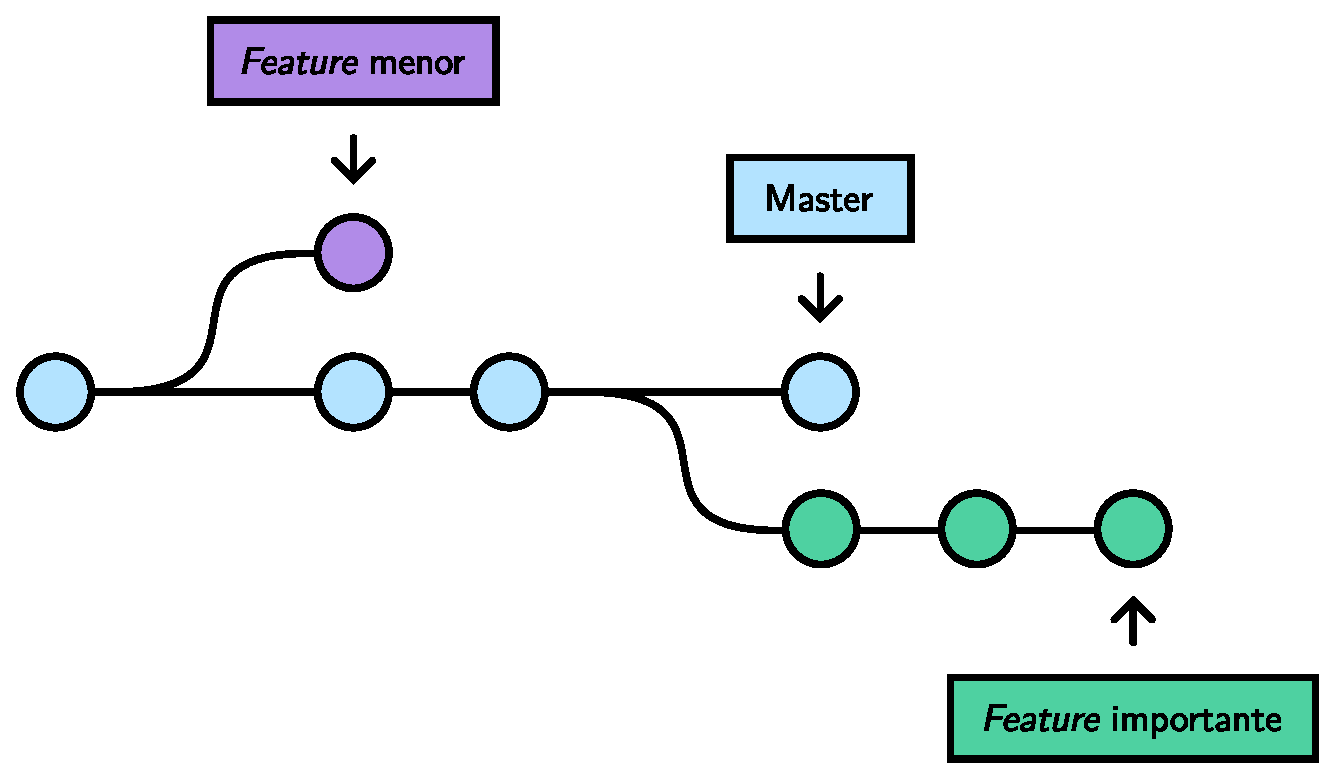
\includegraphics[height=1.5in]{images/branch.pdf}
        \end{center}
    \end{figure}

    % \only<3-3>{
    %     \begin{figure}[ht]
    %         \begin{center}
    %             \includegraphics[height=1.5in]{images/branch-1.png}
    %         \end{center}
    %         \caption{La rama ``master'' apunta al commit \textit{f30ab}}
    %     \end{figure}
    % }
    %
    % \only<4-4>{
    %     \begin{figure}[ht]
    %         \begin{center}
    %             \includegraphics[height=1.5in]{images/branch-2.png}
    %         \end{center}
    %         \caption{Creamos una nueva rama llamada ``testing''}
    %     \end{figure}
    % }


    % Ademas de tener ramas locales, podemos tenemos ramas remotas, que referencian al estado de ramas en tus repositorios remotos.
    % Si por ejemplo quisieramos saltar a la rama ``master'' en el repositorio remoto ``origin'' podríamos utilizar el comando \texttt{git checkout origin/master}.
    %
    % \vspace{1em}
    %
    % Nuestras ramas locales no sincronizan automaticamente con los repositorios remotos. Por esta razón, si tenemos una rama llamada ``master'' de forma local que
    % apunta a la rama remota ``origin/master'' podemos actualizarla parandonos en ``master'' y ejecutando \texttt{git pull origin master}.
    %
    % \vspace{1em}
    %
    % De forma análoga, si queremos publicar cambios locales aun repositorio remoto, tenemos el comando \texttt{git push}. Si estamos parados en la rama ``master'':
    % \texttt{git push origin master}.

\end{frame}

\begin{frame}[t]{Creando ramas}
    \begin{comando}
        git branch
    \end{comando}

    \pause
    \begin{block}{}
        Para crear una rama nueva, podemos ejecutar \texttt{git branch [nombre de la rama]}.

        \vspace{.4em}

        Nótese que este comando no nos mueve a la nueva rama, solo la crea.

        \vspace{.4em}

        Para ver las ramas de nuestro repositorio local, podemos ejecutar \texttt{git branch}.
    \end{block}

    \pause
    \begin{ejercicio}{Ejercicio}
        Crear una rama llamada ``prueba'' en algún repo de la clase pasada.
    \end{ejercicio}

\end{frame}

\begin{frame}[t]{Cambiando de rama}
    \begin{comando}
        git checkout
    \end{comando}

    \pause
    \begin{block}{}
        Para cambiar de rama, podemos ejecutar \texttt{git checkout [nombre de la rama]}.
    \end{block}

    \pause
    \vspace{0.5em}
    Un ejemplo visual:
    \vspace{-1.6em}

    \only<3-3>{
        \begin{figure}[ht]
            \begin{center}
                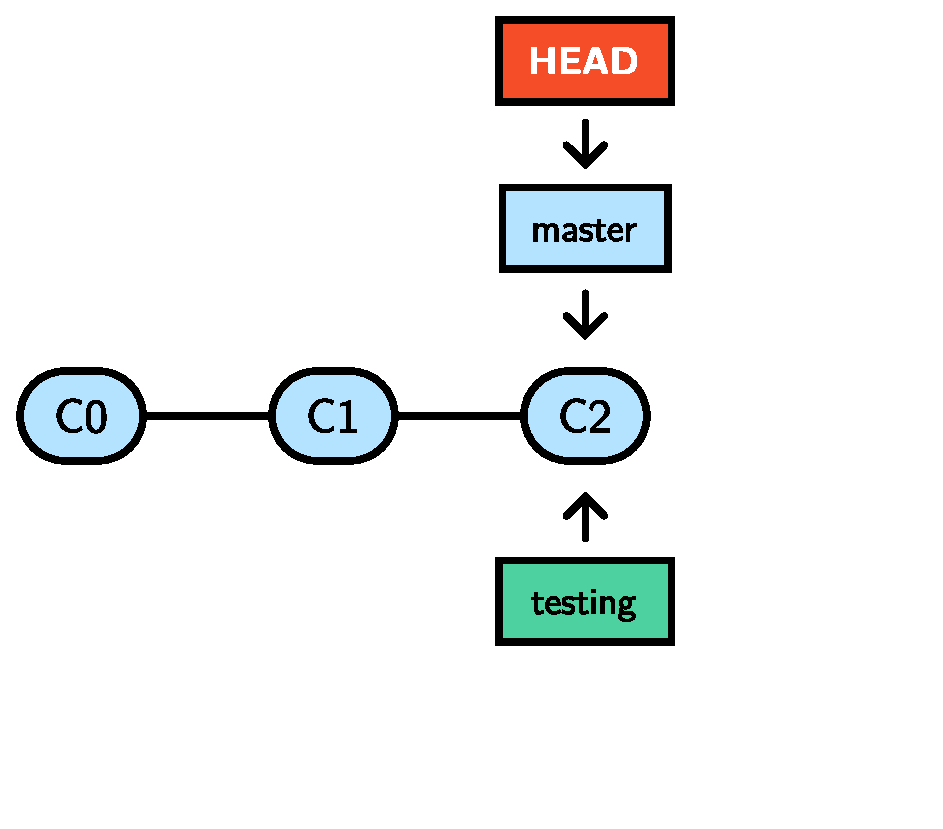
\includegraphics[height=1.6in]{images/checkout-branch-0.pdf}
            \end{center}
            \caption{}
        \end{figure}
    }

    \only<4-4>{
        \begin{figure}[ht]
            \begin{center}
                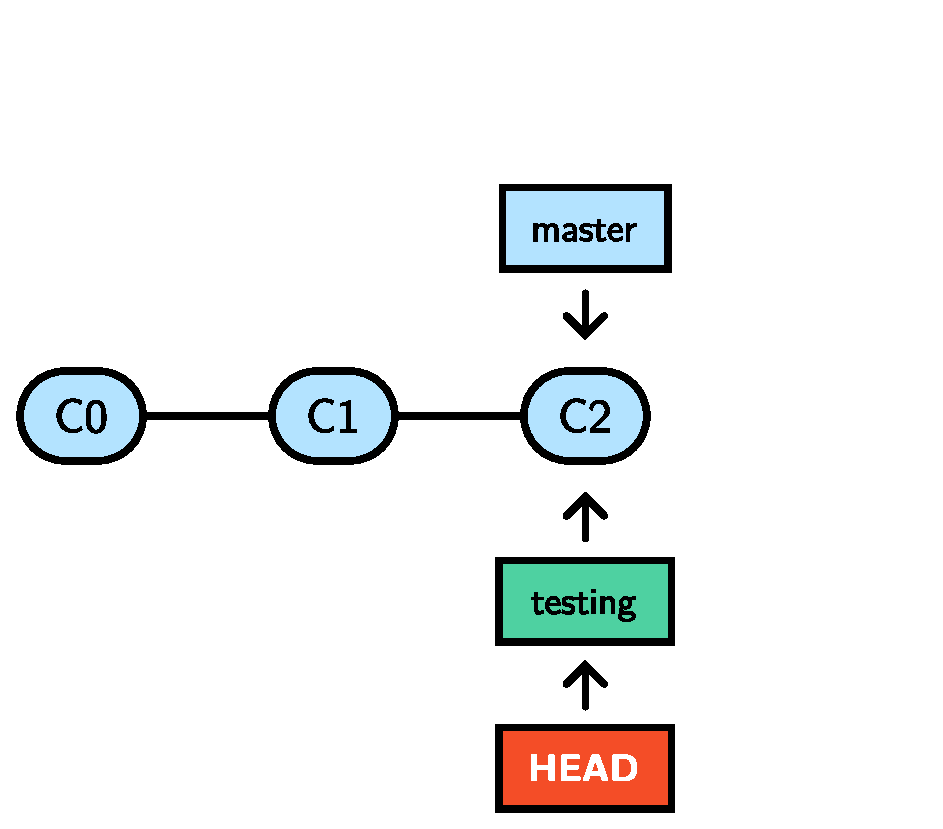
\includegraphics[height=1.6in]{images/checkout-branch-1.pdf}
            \end{center}
            \caption{Acá cambiamos a la rama ``testing'', ejecutando \texttt{git checkout testing}.}
        \end{figure}
    }

    \uncover<5-5>{
        \begin{figure}[ht]
            \begin{center}
                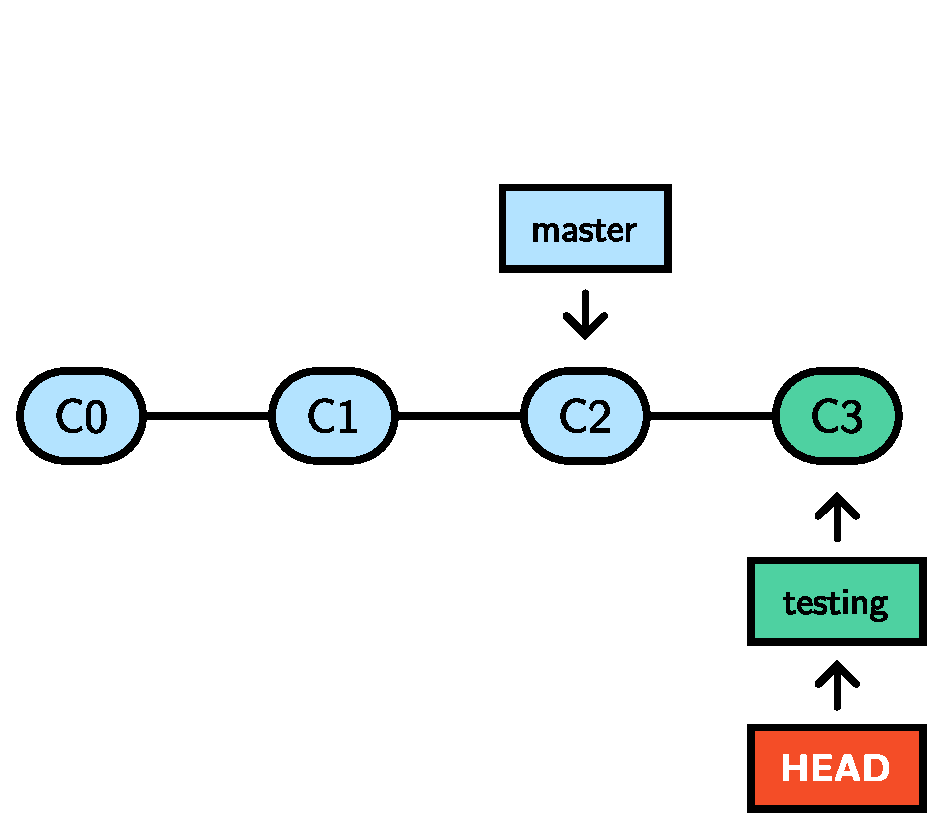
\includegraphics[height=1.6in]{images/checkout-branch-2.pdf}
            \end{center}
            \caption{Y los siguientes \textit{commits} serán agregados a la rama ``testing''.}
        \end{figure}
    }

\end{frame}

\begin{frame}[t]{Fusionando ramas}
    \begin{comando}
        git merge
    \end{comando}

    \pause
    \only<2-2>{
        \begin{block}{}
            Nos permite fusionar las historias de dos ramas distintas (podría haber conflictos).

            \vspace{.4em}

            La sintaxis es: \texttt{git merge [nombre de la rama a fusionar]}.

            \vspace{.4em}

            \textbf{Importante:} este comando fusiona la rama que le decimos
            \textbf{en la rama en la que estamos parados}.
        \end{block}
    }

    \pause
    Un ejemplo visual:
    \only<3-3> {
        \begin{figure}[ht]
            \begin{center}
                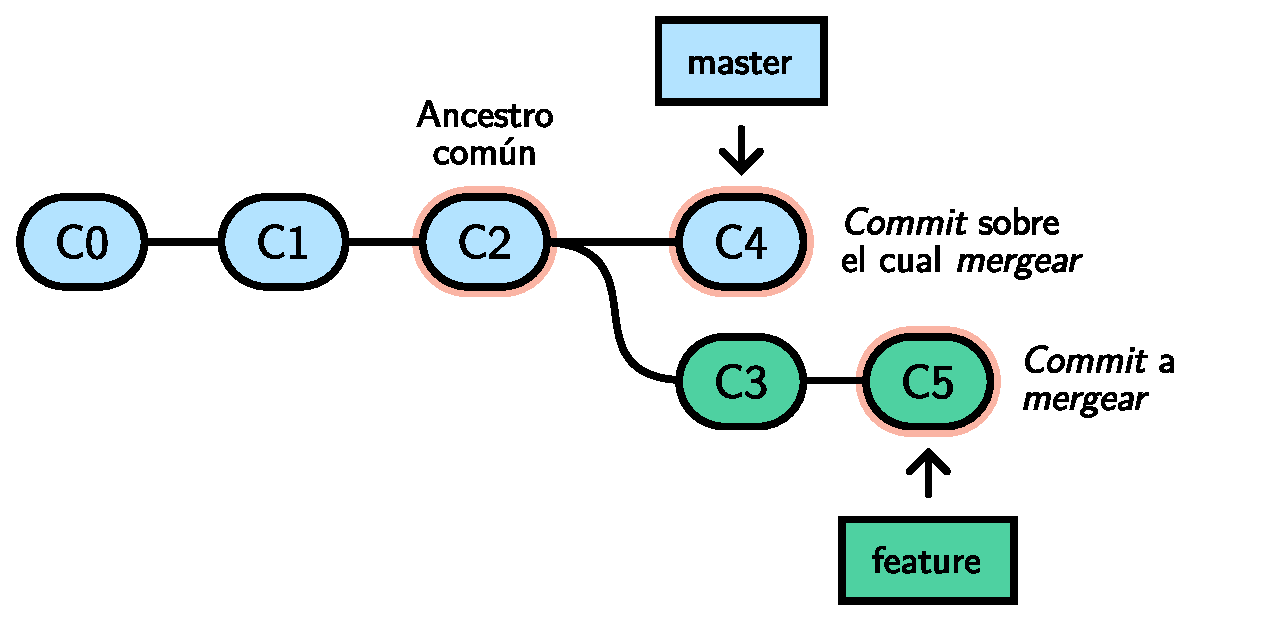
\includegraphics[height=1.5in]{images/merge-branch-0.pdf}
            \end{center}
            \caption{Antes del \textit{merge}.}
        \end{figure}
    }
    \only<4-4> {
        \begin{figure}[ht]
            \begin{center}
                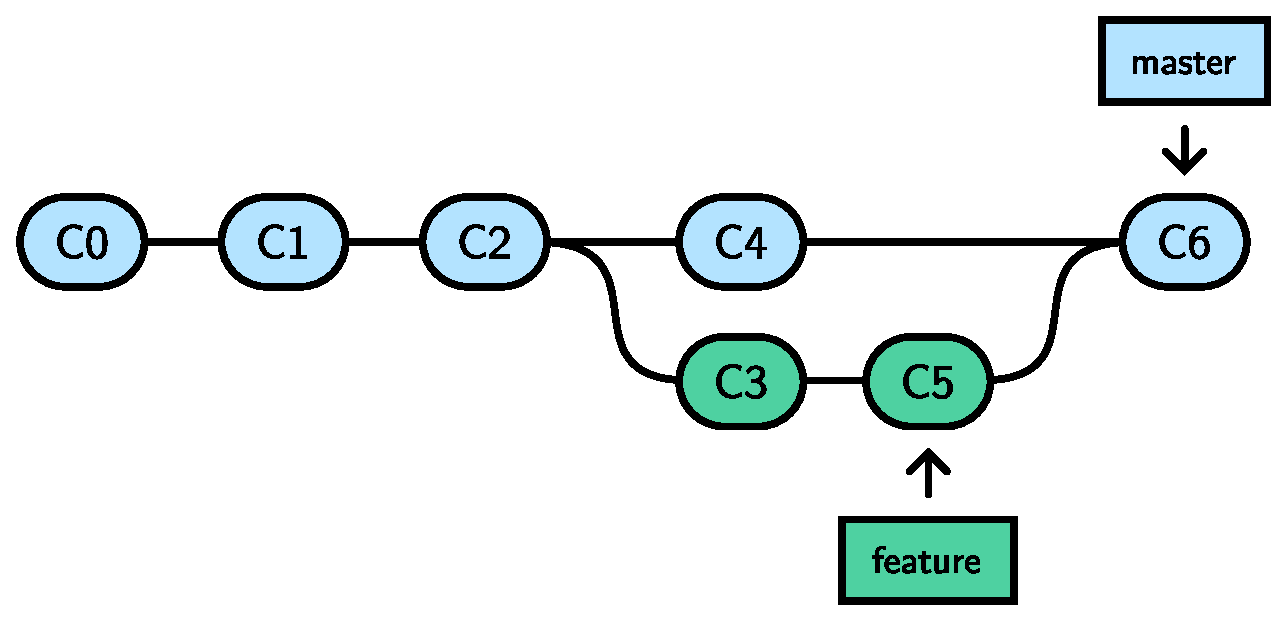
\includegraphics[height=1.5in]{images/merge-branch-1.pdf}
            \end{center}
            \caption{Después de pararnos en la rama ``master'' (\texttt{git checkout master}) y haber fusionado la rama ``feature'' (\texttt{git merge feature}).}
        \end{figure}
    }
\end{frame}

\begin{frame}[t]{¡A practicar!}

    \pause
    \begin{block}{Pero antes de empezar...}
        Para hacer el siguiente ejercicio, vamos a trabajar con un \textbf{fork} de un repositorio.
        \pause\textit{¿Y eso?}

        \pause
        El concepto de \textit{fork} no es propio de Git. En el ámbito del desarrollo de software,
        el término se refiere a un proyecto que surge a partir de otro, y adopta un curso de
        desarrollo independiente.

        \pause
        Los servidores de Git, como GitLab, nos permiten hacer \textit{fork} de proyectos. Al hacer
        esto creamos una copia de un repositorio ajeno en nuestra propia cuenta, sobre la cual
        podemos trabajar libremente. Los cambios que hagamos en nuestra copia \textbf{no} impactarán
        en el repositorio original.
    \end{block}

    \pause
    \begin{center}
    \Large Ahora sí...
    \end{center}
\end{frame}

\begin{frame}[t]{¡A practicar!}
    \begin{ejercicio}{Ejercicio de a 2 máquinas (preferiblemente 2 personas): 👾 y 👽}
        \begin{enumerate}\begin{scriptsize}
            \pause
            \item 👽: Hacer un \textit{fork} en su cuenta de \href{https://www.gitlab.com}{GitLab}
            de este repositorio: \url{https://gitlab.com/talleres-comcom/taller-git-ejercicio2}, y darle permiso a 👾
            para hacer \textit{push}.
            \pause
            \item 👾 y 👽: Obtener una copia local del repositorio de 👽.
            \pause
            \item 👾 y 👽: El repo tiene una única rama, ``master'', donde van a encontrar la letra,
            incompleta, de \href{https://youtu.be/dDq0ne1xK3o}{una canción}. Repartirse el trabajo:
            uno deberá completar la parte A y el otro, la parte B.
            \pause
            \item 👾 y 👽: Crear, cada uno, una rama propia donde harán sus modificaciones. Posicionarse
            en la rama recién creada.
            \pause
            \item 👾 y 👽: Completar la parte elegida de la canción, y hacer \textit{push} de estos
            cambios en el repositorio remoto.
            \pause
            \item 👾: Crear una nueva rama \textbf{a partir de ``master''} con el nombre que 👽 usó para
            la suya, y traerse (\textit{pull}) a esta rama los cambios de 👽.
            \pause
            \item 👾: Volver a su rama de trabajo y fusionar en ella los cambios de 👽. Enviar estos
            cambios al repositorio remoto.
            \pause
            \item 👽: Seguir los dos pasos anteriores, pero con los cambios de 👾.
        \end{scriptsize}\end{enumerate}
    \end{ejercicio}

\end{frame}

\begin{frame}[t]{Revirtiendo cambios}
    \begin{comando}
        git commit --amend
    \end{comando}

    \uncover<2->{
        \begin{block}{}
            Podemos usarlo para \textbf{arreglar}, por ejemplo, el mensaje del último \textit{commit} que hicimos: \texttt{git commit --amend -m [nuevo mensaje]}.
        \end{block}
    }

    \vspace{2em}

    \begin{comando}
        git revert
    \end{comando}

    \uncover<3->{
        \begin{block}{}
            Permite \textbf{revertir} exactamente los cambios introducidos por un \textit{commit}. Buscamos el \textit{hash} del \textit{commit} en cuestión
            usando \texttt{git log}, y luego ejecutamos \texttt{git revert [hash]}.
        \end{block}
    }
\end{frame}

\begin{frame}[t]{Otro comando útil}
    \begin{comando}
        git stash
    \end{comando}

    \pause
    \begin{block}{}
        Al ejecutar \texttt{git stash}, se guarda el estado actual de los archivos modificados y nos deja el directorio limpio.

        \vspace{0.5em}

        Para volver a mostrar los cambios guardados ejecutamos \texttt{git stash apply}.
    \end{block}
\end{frame}

\begin{frame}[t]{Extras: Ignorando archivos}

    \begin{block}{El archivo .gitignore}
      Es común tener archivos generados automáticamente que no queremos agregar al repositorio. Por ejemplo, archivos compilados: .pdf, .exe, .log, .pyc, etc. Sin embargo, es bastante molesto verlos todo el tiempo al ejecutar \texttt{git status}.

      Para arreglar esto podemos crear un archivo especial llamado \texttt{.gitignore}, que le indica a Git qué archivos \textbf{ignorar} por completo.
    \end{block}

    \pause
    \begin{resumen}{}
      Por ejemplo, para ignorar todos los archivos con extensión \textit{.pyc}:
      \begin{enumerate}
        \item Crear un archivo llamado \texttt{.gitignore} en el directorio principal del proyecto.
        \item Adentro escribir: \textit{*.pyc}
      \end{enumerate}
      Más ejemplos de \texttt{.gitignore}: \url{https://github.com/github/gitignore}.
    \end{resumen}


\end{frame}

\begin{frame}[t]{Extras: Más comandos}

    \begin{itemize}
        \item \texttt{git fetch [remote repository]}: Para traer todos los datos de un repositorio remoto.
        \item \texttt{git reset}: Permite deshacer cambios; sirve para revertir modificaciones en el área de trabajo, pero también puede eliminar por completo \textit{commits} anteriores. ¡Usar con mucho cuidado!
        \item \texttt{git rebase [branch]}: Aplica todos los \textit{commits} que difieren entre una rama y aquella en la que estamos parados. Así podemos incorporar cambios realizados en otras ramas manteniendo lineal el historial de la rama actual.
        \item \texttt{git blame [archivo]}: Para ver qué \textit{commit} modificó por última vez cada línea de un archivo, y quién fue su autor. ¡Así, podemos saber a quién \textit{culpar} cuando haya problemas!
        \item \texttt{git bisect}: Encuentra cuál fue el \textit{commit} que introdujo cierto error, haciendo búsqueda binaria en el historial de \textit{commits}.
    \end{itemize}

\end{frame}

\begin{frame}[t]{Extras: Servidores}

    \begin{figure}[ht]
        \begin{center}
            
\includegraphics[height=0.7in]{images/github.png}
        \end{center}
    \end{figure}

    \begin{figure}[ht]
        \begin{center}
            
\includegraphics[height=0.5in]{images/bitbucket.png}
        \end{center}
    \end{figure}

    \begin{figure}[ht]
        \begin{center}
            
\includegraphics[height=0.7in]{images/gitlab.png}
        \end{center}
    \end{figure}

\end{frame}

\begin{frame}[t]{Bibliografía}

    \begin{itemize}
        \item Git Community book, disponible online y en español: \url{https://git-scm.com/book/es/v2}
        \item \texttt{git help [command]} para ver la documentación de cualquier comando de Git.
        \item A visual Git reference: \url{http://marklodato.github.io/visual-git-guide/index-es.html}
        \item Try Git online: \url{https://try.github.io}
    \end{itemize}

\end{frame}

\begin{frame}{Feedback}

    \begin{center}
        
\includegraphics[height=1.5in]{images/octocat-comcom.pdf}
    \end{center}

    \begin{block}{¡Nos interesa saber que les pareció el taller!}
        Pueden completar el formulario: \url{https://goo.gl/forms/LUnKy5kmPJmYAeer1}

        \vspace{0.5em}

        También nos pueden tirar ideas para futuros talleres.
    \end{block}

\end{frame}
